% ==============================================================
% --- Git
% ==============================================================
\section{Automated Version Control}\hypertarget{sec1}{}
\setcounter{framenumber}{0}

\begin{frame}[fragile]
\frametitle{Why version control?}

  \begin{columns}

    \begin{column}{0.6\textwidth}
      Problems
      \begin{itemize}
        \small
        \item Multiple, nearly identical versions of the same document
        \item Tracking changes is not an option for source code
        \item No protection against accidental deletion
      \end{itemize}
      \vspace{0.15cm}
      Version control systems 
      \begin{itemize}
        \small
        \item {\bf start} with a base version of the document
        \item {\bf record} changes you make each step of the way
        \item can {\bf revert} to any previous versions if necessary
        \item {\bf never lose} a previous state of your document
        \item allow many people to {\bf work in parallel}
      \end{itemize}
    \end{column}

    \begin{column}{0.4\textwidth}
    \begin{figure}[h]
    
\includegraphics[width=0.9\textwidth]{sec1/comic_version_control.png}
    \end{figure}
    \end{column}

  \end{columns}

\end{frame}

\begin{frame}[fragile]
\emptyframetitle
  \begin{columns}
    \begin{column}{0.33\textwidth}
{\bf Sequential changes}
      \begin{figure}[h]
      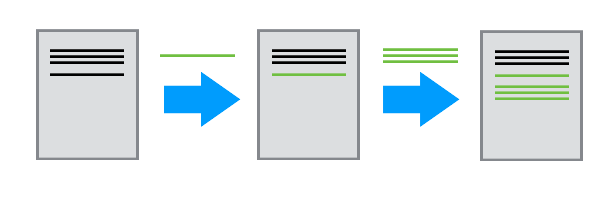
\includegraphics[width=1.0\textwidth]{sec1/change.png}
      \end{figure}
      Start at the base document, apply each change, arrive at the more recent version
    \end{column}
    \begin{column}{0.33\textwidth}
{\bf Diverging versions}
      \begin{figure}[h]
      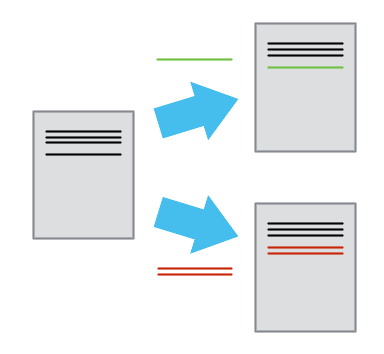
\includegraphics[width=1.0\textwidth]{sec1/versions.png}
      \end{figure}
      Two users can make independent sets of changes on the same document
    \end{column}
    \begin{column}{0.33\textwidth}
{\bf Merge versions}
      \begin{figure}[h]
      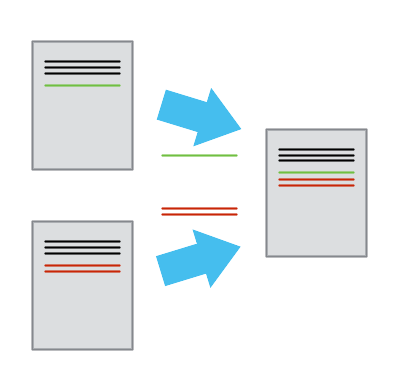
\includegraphics[width=1.0\textwidth]{sec1/merge.png}
      \end{figure}
      Incorporate two sets of changes into the same base document
    \end{column}

  \end{columns}

\end{frame}

\begin{frame}[fragile]
\emptyframetitle

\textbf{Further reasons} for using Git

\begin{itemize}
\setlength\itemsep{10pt}
  \item \textbf{Sequence of clean, logical patches}, not uncorrelated random changes
  \item Git as starting point for \textbf{automated unit and regression tests}, e.g. via Gitlab, GitHub
  \item Git for \textbf{reproducing results}, not only source code
  \begin{itemize}
    \normalsize
    \item configuration changes
    \item data sets
    \item anything in ASCII
    \item \LaTeX source code
  \end{itemize}
  \item \textbf{Collaboration} as everyone uses Git
\end{itemize}
\end{frame}

\begin{frame}[fragile]
\emptyframetitle

Example: determine buggy version via bisection\\[7pt]

\textbf{Manually}
\begin{enumerate}
  \item Define (latest) buggy version \texttt{B}
  \item Find some working version \texttt{W}
  \item Check out intermediate version \texttt{I} half-way between \texttt{B} and \texttt{W}, build, run\label{int_man}
  \begin{itemize}
    \normalsize
    \item Working? $\Rightarrow$ \texttt{W = I}
    \item Not working? $\Rightarrow$ \texttt{B = I}
  \end{itemize}
  \item Goto \ref{int_man}
  \item Identfied buggy version?
  \begin{itemize}
    \normalsize
    \item Identify change that causes the bug
    \item Do \texttt{diff} on \textbf{all} source code files
    \item \textbf{Can take hours, days or weeks} depending on code size and differences
  \end{itemize}
\end{enumerate}

\end{frame}

\begin{frame}[fragile]
\emptyframetitle

Another example: determine buggy version via bisection\\[7pt]

\textbf{Automated}
\begin{enumerate}
  \item Start bisect wizzard with \texttt{git bisect start}
  \item Define buggy version with \texttt{git bisect bad someCommitID}
  \item Define working version with \texttt{git bisect good anotherCommitID}
  \item Git checks out intermediate version, build, run\label{int_aut}
  \begin{itemize}
    \normalsize
    \item Working? $\Rightarrow$ \texttt{git bisect good}
    \item Not working? $\Rightarrow$ \texttt{git bisect bad}
  \end{itemize}
  \item Git goes to \ref{int_aut}
  \item Identfied buggy version?
  \begin{itemize}
    \normalsize
    \item \textbf{Read associated change}
    \item \textbf{Takes seconds!}
  \end{itemize}
\end{enumerate}


\end{frame}

